%% A simple template for a lab or course report using the Hagenberg setup
%% based on the standard LaTeX 'report' class

%%% Magic comments for setting the correct parameters in compatible IDEs
% !TeX encoding = utf8
% !TeX program = pdflatex 
% !TeX spellcheck = en_US
% !BIB program = biber

\RequirePackage[utf8]{inputenc} % Remove when using lualatex or xelatex!
\RequirePackage{hgbpdfa}	


% Remove if NO PDF/A output is desired

\documentclass[english,notitlepage,smartquotes]{hgbreport}
% Supported options in [..]:
%    Main language: 'german' (default), 'english'
%    Conversion to typographic quotation marks: 'smartquotes'
%    Use APA citation style: 'apa'
%    Do not create a separate title page: 'notitlepage'
%    Page layout: 'oneside' (single-sided, default), 'twoside' (double-sided)
%%%-----------------------------------------------------------------------------


\renewcommand{\chaptername}{Lab}

\graphicspath{{images/}}     % Location of images and graphics
\bibliography{hgbreferences}    % Biblatex bibliography file (hgbreferences.bib)
\ExecuteBibliographyOptions{backref=false} % No back references in bibliography

%%%-----------------------------------------------------------------------------
	% <----- set to assignment number!
%%%-----------------------------------------------------------------------------
\begin{document}
%%%-----------------------------------------------------------------------------

\author{Simone Bianca\ Feldbacher}                      % Your name
\title{DRS MC508 -- SS 2025\\ % Name of the course
				Lab Report Exercises 1--8} % Title of the report
\date{\today}

%%%-----------------------------------------------------------------------------
\maketitle
%%%-----------------------------------------------------------------------------

\begin{abstract}\noindent
The Course Distributed Real Time Systems focuses on the principles and
technologies for building distributed real-time systems. The course covers fundamental topics like worst-case execution time analysis, real-time communication, scheduling algorithms, resources, and comunication. These concepts are applied using QNX 8 on a raspberry Pi 4. 
This report summarizes the 8 assignments completed during the course, highlighting the key concepts and techniques learned in each chapter. 

\end{abstract}


\tableofcontents
\cleardoublepage
%%%-----------------------------------------------------------------------------

\chapter{Assignment 1 --- WCET}

\section{Assignment}
After learning about scheduling and worst-case execution time (WCET) analysis, the first assignment focuses on developing a simple real-time application and analyzing its scheduling behavior and WCET. A passenger protection system is a system that has strong requirements for real time and fault tolerance. The following tasks should be completed: 
\begin{itemize}
    \item Implement a simplified version of the Airbag Deployment Algorithm described in \cite{mahmudNewDecisionMaking1995}. Using either C or C++, Don't use floating point numbers or OO features. 
    \item Analyze the WCET using IAR embedded workbench.
    \item Use BoundT to analyze the WCET. compare both results.
\end{itemize}

\section{Implementation}
The provided paper and lecture slides provide a starting point and outline how to implement the airbag deployment algorithm. 
It works by consistently calculating the current change in velocity as well as the length of the acceleration graph. Based in these values the system enters a STANDBY state and fires the airbag if the right conditions are met. 
Three thresholds are defined:  
\begin{itemize}
    \item $\Delta V_1$: The change in velocity must be greater than $\Delta V_1$ to enter the STANDBY state.
    \item $\Delta V_2$: If change in velocity exceeds this value the airbag is fired immediately. $\Delta V_2$ must be greater than $\Delta V_1$.
    \item $L$: The length of the acceleration graph must be greater than $L$ during standby state to fire the airbag.
\end{itemize}

Before implementation the algorithm was broken down into steps and states as follows: 

\subsection{Initialization} Sliding windows are initialized as arrays of size $N$ and filled with zeros. The system starts in the \emph{NORMAL} state. Everything after this is executed in an endless loop. Rudimentary timing is implemented using \texttt{usleep(1000000 / SAMPLES\_PER\_SECOND)}.

\begin{CCode}
    // Initialize arrays for storing time samples
    int t1[T_SIZE1] = {0}; // Array for first time series
    int t2[T_SIZE2] = {0}; // Array for second time series

    // Define thresholds for change in velocity
    int deltaV1 = 20; // Threshold for entering standby state
    int deltaV2 = 50; // Threshold for firing the airbag
    int LThreshold = 300; // Threshold for length of acceleration graph

    // Variables for current calculations
    int deltaV = 0; // Current change in velocity
    int L = 0; // Current length of acceleration graph

    // Variable to hold the current sample index
    int currentSample;

    // State of the airbag system
    AirbagState state = NORMAL; // Initial state is NORMAL
\end{CCode}

\subsection{Data Acquisition} Query new data, random values in this case, and update the sliding windows by shifting existing values and adding the new data. This step happens regardless of state. 

\begin{CCode}
    static void processSample(int t1[], int size1, int t2[], int size2, int *deltaV, int *L)
    {
    int currentSample = rand() % (10 + 1 + 30) - 30;
    printf("Current Sample: %d\n", currentSample);

    slideWindow(t1, size1, currentSample);
    slideWindow(t2, size2, currentSample);

    *deltaV = determineDeltaV(t1, size1);
    *L = determineL(t2, size2);

    printf("DeltaV: %d, L: %d\n", *deltaV, *L);
}

\end{CCode}

\subsection{Calculation} Calculate $\Delta V$ and $L$ within the scope of the sliding windows, using the formulas presented in the paper. 

\begin{CCode}
    static int determineDeltaV(int window[], int size)
    {
    double deltaV = 0;

    for (int i = 0; i < size; i++)
    {
        deltaV += window[i] * 1.0 / SAMPLES_PER_SECOND;
    }
    return round(deltaV);
}

static int determineL(int window[], int size)
    {

    double l = 0, dy = 0;
    double dx = 1.0 / SAMPLES_PER_SECOND;
    for (int i = 0; i < size - 1; i++)
    {
        dy = window[i + 1] - window[i];
        l += sqrt(pow(dy, 2) + pow(dx, 2));
    }
    return (int)l;
}
\end{CCode}

\subsection{State Transition} Possible states are \emph{NORMAL}, \emph{STANDBY} and \emph{FIRE}. If $\Delta V$ exceeds $\Delta V_1$ the system enters the standby state. If $\Delta V$ exceeds $\Delta V_2$ the system fires immediately. If the system is in STANDBY state and $L$ exceeds the threshold $L$, the system fires. If the system is in STANDBY state and $\Delta V$ drops below $\Delta V_1$ the system goes back to normal. For clarity these are implemented as switch cases.

Possible transitions are: 
\begin{itemize}
\item NORMAL $\rightarrow$ STANDBY $\rightarrow$ NORMAL 
\item NORMAL $\rightarrow$ STANDBY $\rightarrow$ FIRE
\end{itemize}

\begin{CCode}
        case NORMAL:
            processSample(t1, T_SIZE1, t2, T_SIZE2, &deltaV, &L);
            if (abs(deltaV) > deltaV1)
            {
                state = STANDBY;
            }
            break;

        case STANDBY:
            processSample(t1, T_SIZE1, t2, T_SIZE2, &deltaV, &L);
            if (abs(deltaV) > deltaV2 || L > LThreshold)
            {
                state = FIRE;
            }
            if (abs(deltaV) < deltaV1)
            {
                state = NORMAL;
            }
            break;

        case FIRE:
            exit(0);
            break;  

\end{CCode}

\subsection{Challenges} 
While the algorithm was simple to implement, trying to run it in the provided version of IAR Embedded Workbench caused some problems. Headers like time.h were not included per default and would have taken up too much space to compile in the free version. std:out was initially replaced with \texttt{printf} and later entirely omitted due to the same space concerns. Some rewrites were necessary to fix these problems.These problems were tackled as follows: 
\begin{itemize}
    \item unsupported headers: Removed time.h since only the WCET of the actual code execution matters for WCET, 
    \item Error e89: Caused by exceeding the 4KB object code limit of the kick start version. Remove the studio.h header to save on object code. This also means removing all \texttt{printf} statements, which did not matter for the WCET analysis anyway.
    \item Error e16: Occurred during building. Was fixed by selecting the \textit{ATmega328P} as the target processor. 
\end{itemize}
BoundT presented it's own set of challenges. It would, despite my best efforts, not compile on my machine so the pre-installed version in the proved VM was used instead. The 1024kb limit was no problem. The require .elf file was compiled from VS code using gcc, which failed due to missing STABS symbols. Using an older version of the compiler and including stabs finally lead to a usable result. 



\section{Evaluation}
After getting \textit{Wayland} and \textit{VMware Workstation} to stop fighting using the true and trust method of copying a fix from Reddit, all the analysis was done on the provided version of Windows XP. 

\begin{figure}[h]
    \centering
    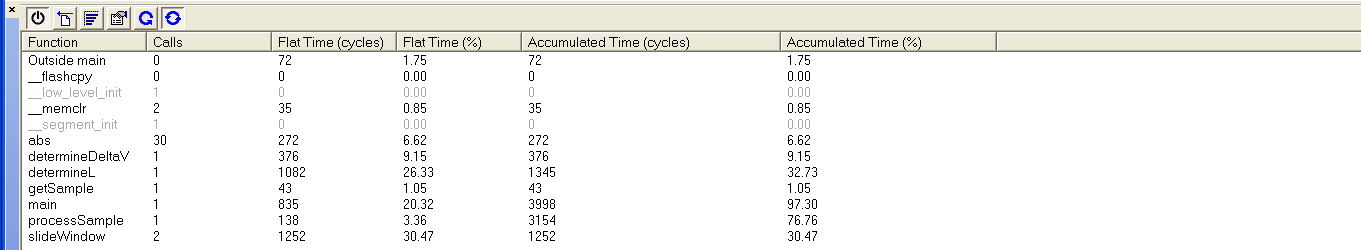
\includegraphics[width=0.9\textwidth]{IAR_02.png}
    \caption{Profiling view from IAR Embedded Workbench Simulator. }
    \label{fig:IAR01}
\end{figure}

\subsection {WCET analysis from the IAR Simulator Results}

Debugging the code in IAR resulted in the following execution times for one loop after the initial setup (seen in \ref{fig:IAR01}) for the function implemented. \texttt{slideWindow} gets called twice per loop because the sliding windows are implemented as two separate arrays. The Accumulated Time for \texttt{main} shows that it takes 3998 cycles to execute one loop. At a clock speed of 16MHz this would take 0.25ms to execute, well under the 30ms requirement for the airbag system. Such a short time is expected because the sensor reading is not accounted for and the sliding windows are small with only a length of 20 and 30 respectively. Increasing both by 10 already increases the time to 5300 cycles or 0.33ms.



\subsection{WCET results from BoundT} 
After compiling the algorithm for the Atmega128 (the Atmega328P was not supported in BoundT) the analysis was run with the following parameters: 

\begin{CCode}
    boundt_avr -device=ATmega128 -elf_sym -max_steps 1024 -show times airbag_atmega128_stabs.elf main 
\end{CCode}

The resulting WCET in CPU cycles were: 
\begin{itemize}
    \item 2386 cycles for the \texttt{processSample} function, which coposes fetching the samples, sliding the windows and calculating $\Delta V$ and $L$.
    \item 3144 cycles for the \texttt{main} function, which includes the state transitions and the calls to \texttt{processSample}. 
\end{itemize}

These results are lower than the ones obtained from the IAR Simulator. This difference could come from the fact that the code was compiled for a different processor, or that the compilation in VS code performed some optimizations that the IAR compiler did not. 

\subsection{Discussion}

For both results it is important to keep in mind that the WCET from this example is not realistic since the code does not include the time it takes to read the sensors, which is a crucial part of the airbag system. The results are only for the processing of a small set of sample data and the state transitions, to satisfy the goal of this assignment which was to get familiar with the tools and the process of WCET analysis.

\chapter{Assignment 2 --- Scheduling policies}

\section{Assignment}
After having determined the WCET for one of the tasks in the airbag system to be about 0.25ms or 250$\mu s$ in the last assignment, now we have to consider other tasks that get executed periodically in the system as well. From the lecture slides the following three additional tasks were selected: 
\label{tab:tasks}
\begin{table}[h]
    \centering
    \caption{Tasks with their periods and worst-case execution times}
    \begin{tabular}{|c|p{6cm}|c|c|}
        \hline
        \textbf{Task} & \textbf{Description} & \textbf{Period} & \textbf{WCET} \\
        \hline
        $\tau_1$ & As determined in the last chapter. This task is responsible for the airbag deployment. & 1ms & 0.25ms \\
        \hline
        $\tau_2$ & Responsible for gathering data from an additional satellite accelerometer. & 1ms & 0.1ms \\
        \hline
        $\tau_3$ & Responsible for verifying the decision of the airbag system. & 1ms & 0.01ms \\
        \hline
        $\tau_4$ & Responsible for communicating with a Diagnostic interface. & 100ms & 5ms \\
        \hline
    \end{tabular}
\end{table}
The goal of assignment 2 is to work with three different scheduling policies and use \textit{Cheddar} to simulate the resulting schedules. For the different policies the following variables should be determined: 

\begin{itemize}
    \item \textbf{Rate Monotonic (RM)}: A priority based strategy that assumes all tasks are periodic with their deadline being this period. Tasks with shorter periods get higher priorities.
    Perform tests in Cheddar to determine if the system is schedulable under this policy. Perform the Liu/Layland and hyperbolic tests. 
    \item \textbf{Round Robin (RR)}: Fair policy that lets tasks execute until they give up control to the scheduler. Determine the necessary time quantum and how many context switches are necessary. Use Cheddar to simulate the resulting schedule. 
    \item \textbf{Cyclic Executive (CE)}: Fair policy that runs all tasks to completion in the same order repeatedly. Determine the minor and major cycle and if a feasible schedule is possible. 
\end{itemize}

\section{Approach}
The exercises were approached in order of complexity, starting with cyclic executive. 
\subsection{Cyclic Executive}
The greatest common divisor of the tasks from \ref{tab:tasks} is one 1ms, which determines the minor cycle. The major cycle, the least common multiple of the task periods is 100ms. 
While $\tau_1, \tau_2$ and $\tau_3$, who get executed every minor cycle, are feasible to execute within one minor cycle since their execution times only add up to 0.36ms, $\tau_4$ cannot be executed within the minor cycle. Its execution time of 5ms alone is greater than one minor cycle, meaning that during its execution the other tasks cannot meet their deadlines. Therefore, a feasible schedule is not possible under the cyclic executive policy.

\subsection{Round Robin}
Since $\tau_4$ takes so long to execute, it must be interrupted so the other tasks get the chance to meet their deadlines. The first three tasks need to be executed every 1ms, but they also need time to execute, so the quantum needs to be smaller than that. A quantum of 0.6 ms would interrupt $\tau_4$ with 0.4 ms left until the deadline of the first three tasks, which is enough for all three of them to execute. 
To verify this, a simulation was run in Cheddar with the following parameters \ref{fig:RRParams}. 

\label{fig:RRParams}
\begin{figure}[htbp]
  \centering
  \begin{tabular}{cc}
    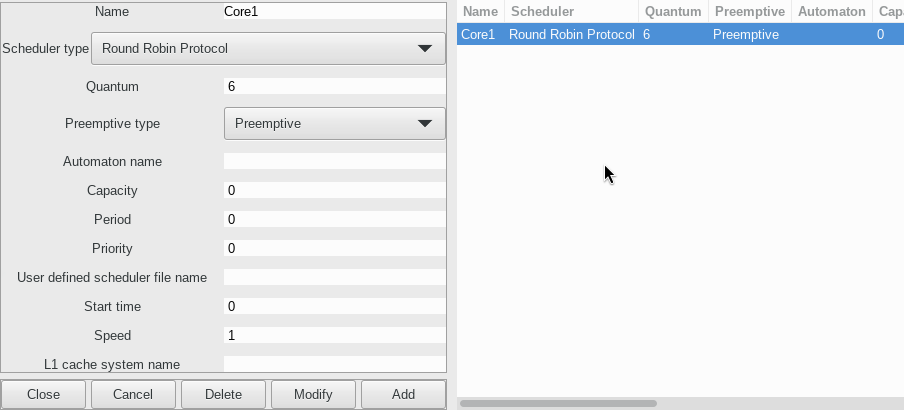
\includegraphics[width=0.48\textwidth]{02_RoundRobin_Core.png} &
    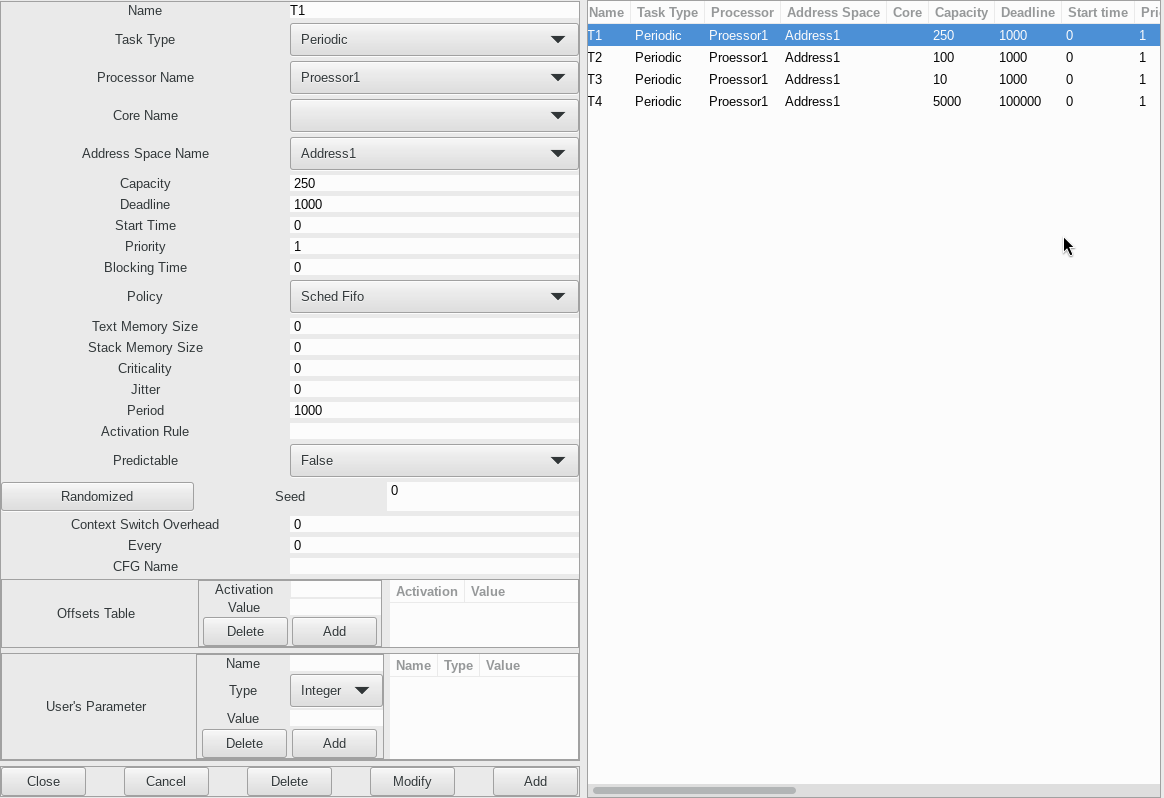
\includegraphics[width=0.48\textwidth]{02_RoundRobin_Tasks.png}
  \end{tabular}
  \caption{Parameters for simulating Round Robin scheduling in Cheddar. The left image shows the core, the right image shows the tasks and their parameters.}
  \label{fig:roundrobin}
\end{figure}

\label{fig:roundrobin}
\begin{figure}[h]
\centering
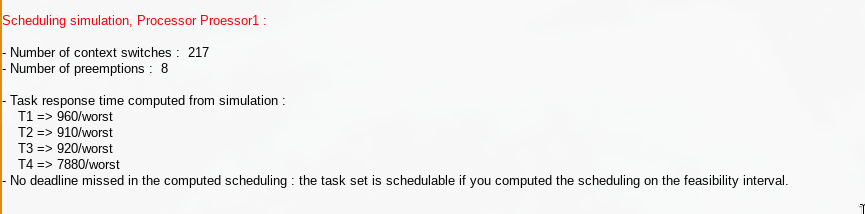
\includegraphics[width=0.7\textwidth]{02_RoundRobin01.png}

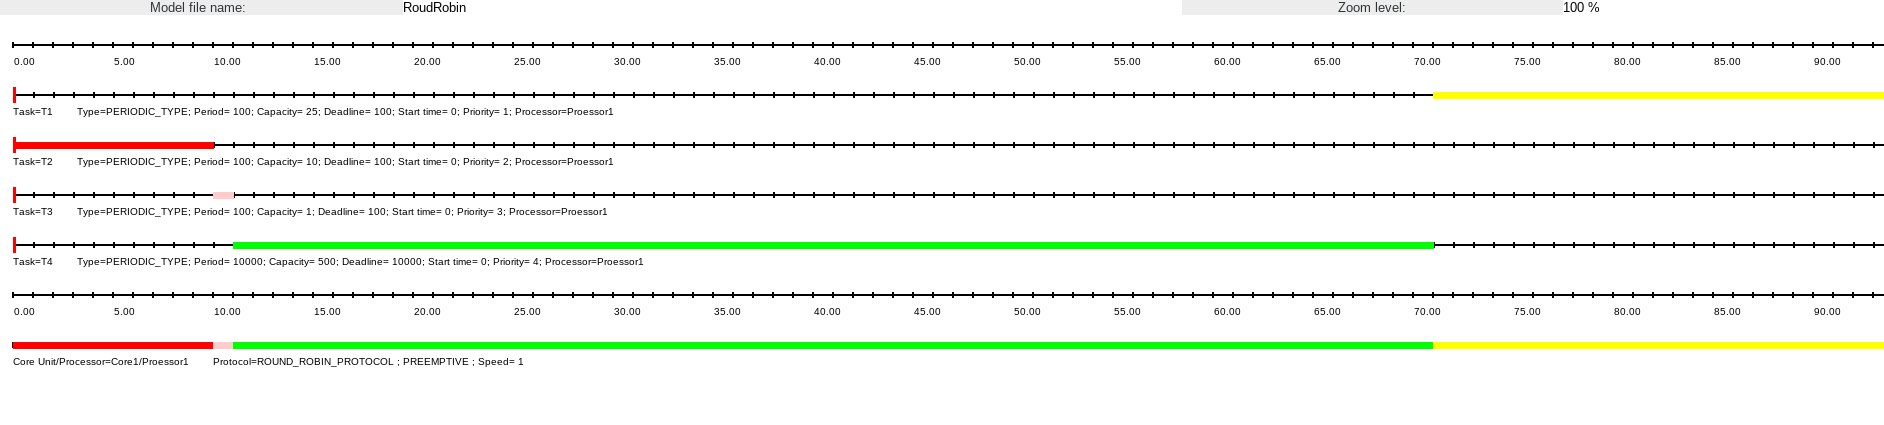
\includegraphics[width=0.7\textwidth]{02_RoundRobin02.png}
\caption{Output from Cheddar for simulating Round Robin scheduling with the parameters from Table \ref{tab:tasks} and a quantum of 0.6ms. Numbers in the top image are in microseconds over the span of 100ms, or one period of task 4. Numbers in the bottom image are multiplied by 100 since Cheddar does not allow for decimal inputs.}
\end{figure}

The simulation confirms that this schedule is feasible but also requires over 200 context switches per 100ms. The high number of context switches is a consequence of the periods and execution time of the tasks varying so greatly. 

\subsection{Rate Monotonic} 

In Rate Monotonic scheduling, the tasks with the shortest period get the highest priority. In this case, $\tau_1, \tau_2$ and $\tau_3$ would have higher priority than $\tau_4$. 

The schedulability condition by Liu and Layland is
\[
U=\sum_{i=1}^{n}\frac{C_i}{T_i}\le n\left(2^{1/n}-1\right),
\]
where \(C_i\) is the (worst-case) execution time of task \(i\), \(T_i\) is the period of task \(i\), and \(n\) is the total number of tasks.

For the tasks from Table \ref{tab:tasks} the utilization \(U\) results in 
\[U = 0.41 \leq 0,76\]
which means that the system is schedulable under the Rate Monotonic policy.

The hyperbolic bound test is given by this condition:
\[
U=\prod_{i=1}^{n}\left(\frac{c_i}{T_i}+1\right)\le 2
\]
which resolves to 
\[U = 1.45 \leq 2\]
meaning this test passes as well. 

To run the simulation in Cheddar, only the schedule type parameter in the core needs to be changed in the setup from the Round Robin simulation. Custom task priorities did not affect the resulting schedule, which is expected since the priorities are determined by the periods of the tasks.
Figure \ref{fig:RM} shows the simulation results. 

\begin{figure}[htbp]

  \centering
  \begin{tabular}{cc}
    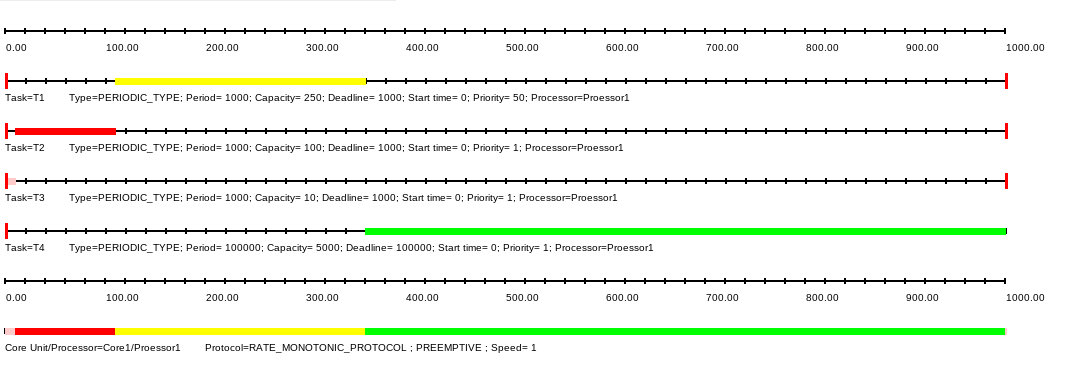
\includegraphics[width=0.48\textwidth]{02_RateMonotonic_timeline.png} &
    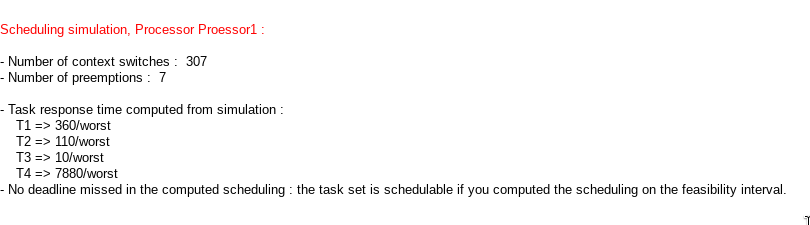
\includegraphics[width=0.48\textwidth]{02_RateMonotonic_result.png}
  \end{tabular}
  \caption{Rate Monotonic scheduling simulation in Cheddar showing the timeline (left) and simulation statistics (right).}
  \label{fig:RM}
\end{figure}

\section{Evaluation}

Table~\ref{tab:scheduling-comparison} shows the simulation results from Cheddar for both scheduling policies over a 100ms interval.
Rate Monotonic scheduling surprisingly results in more context switches than Round Robin, yet it also decreases the WCET for the first three tasks significantly. This is because $\tau_4$ gets preempted more often, which allows the other tasks to execute sooner. The number of preemptions is similar for both policies, which is expected since $\tau_4$ needs to be preempted at least 7 times to allow the other tasks to execute.

\begin{table}[htbp]
    \centering
    \caption{Comparison of Round Robin and Rate Monotonic scheduling simulation results}
    \label{tab:scheduling-comparison}
    \begin{tabular}{|l|c|c|}
        \hline
        \textbf{Metric} & \textbf{Round Robin} & \textbf{Rate Monotonic} \\
        \hline
        Context switches & 217 & 307 \\
        \hline
        Preemptions & 8 & 7 \\
        \hline
        $\tau_1$ response time (worst) & 960\,$\mu$s & 360\,$\mu$s \\
        \hline
        $\tau_2$ response time (worst) & 910\,$\mu$s & 110\,$\mu$s \\
        \hline
        $\tau_3$ response time (worst) & 920\,$\mu$s & 10\,$\mu$s \\
        \hline
        $\tau_4$ response time (worst) & 7880\,$\mu$s & 7880\,$\mu$s \\
        \hline
        Deadlines missed & 0 & 0 \\
        \hline
        Schedulable & Yes & Yes \\
        \hline
    \end{tabular}
\end{table}


\chapter{Assignment 3 - WCET calculator}

\printbibliography[heading=noheader]

%%%-----------------------------------------------------------------------------
\end{document}
%%%-----------------------------------------------------------------------------
